\chapter{الأمينات ومركبات النيتروجين}\label{ch:b2:amines}

السمك الذي لم يعد طازجًا تفوح منه رائحة ثلاثي ميثيل أمين، وهو أمين صغير متطاير.
وعصرة ليمون تزيل الرائحة: فالحمض يبرتن الأمين، وأيون
الأمونيوم المتكوّن، لكونه أيونًا، لا يستطيع التبخر. والزوج الحر للنيتروجين
يجعل الأمينات قواعد ومحبات للنواة؛ وحين يرتبط بكربونيل يعطي الإيمينات،
التي تجري البروتينات عبرها كيمياءها ويصنع الكيميائيون بها الأمينات؛ وعلى
حلقة \omterm{def:b2:huckel:aromatic}{عطرية} يفتح، عبر أملاح الديازونيوم، الطريق إلى أصباغ الآزو
التي لوّنت القرن التاسع عشر.

\begin{recall}
مجلد السنة الأولى: أحماض برونستد وقواعده، و$\mathrm pK_a$ ومخططات الهيمنة،
والمحبات للنواة والاستبدال الثنائي الجزيئية، ونصف الأسيتالات والأسيتالات، ومانحات الهيدريد،
والكواشف العضوية المغنيزيومية، وصنف الكربون. و\cref{ch:b2:aromatic-substitution}:
النترتة، واختزال النتروأرينات. والمجلد المدرسي: الأمينات والأميدات.
\end{recall}

\begin{omfigure}
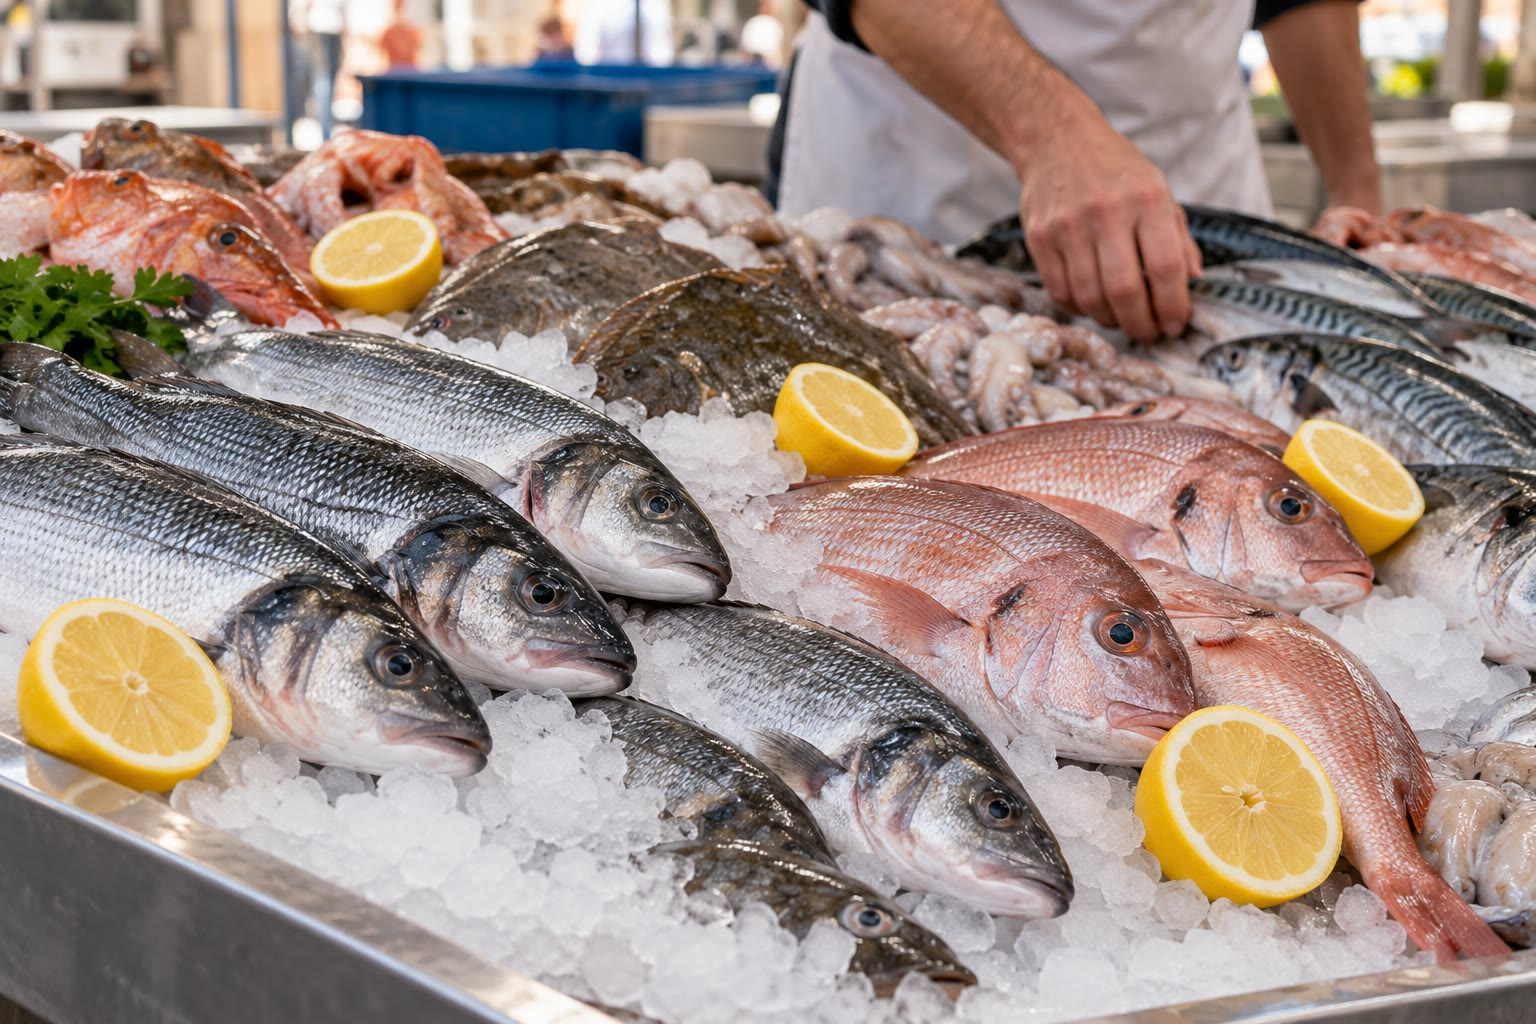
\includegraphics[width=0.6\linewidth]{images/book3/ai/b2-23-fish-stall.jpg}

{\small كشك سمك: أنصاف ليمون موضوعة بين الأسماك. يحوّل حمضها
ثلاثي ميثيل الأمين في السمك إلى أيون أمونيومه غير المتطاير.}
\end{omfigure}

\section{البنية والقاعدية}

\begin{definition}[أصناف الأمينات]\label{def:b2:amines:class}
الأمين إما \emph{أمين أولي}\index{أمين أولي} \ce{RNH2}، وإما \emph{أمين ثانوي}
\index{أمين ثانوي} \ce{R2NH} وإما \emph{أمين ثالثي}\index{أمين ثالثي}
\ce{R3N} بحسب عدد المجموعات الكربونية المرتبطة بالنيتروجين. و\emph{أيون الأمونيوم
الرباعي}\index{أيون أمونيوم رباعي} \ce{R4N+} له أربع منها، ولا زوج حر له.
\end{definition}

نيتروجين الأمين رباعي الأوجه تقريبًا، يشغل الزوج الحر الموضع
الرابع. \omterm{def:b2:amines:class}{والأمين الثالثي} ذو المجموعات الثلاث المختلفة كيرالي من حيث المبدأ لكن لا يمكن
فصله: فالجزيء ينقلب عبر ترتيب مستوٍ، كمظلة في الريح،
آلاف الملايين من المرات في الثانية في درجة حرارة الغرفة.

\begin{proposition}[القاعدية]\label{prop:b2:amines:basicity}
في الماء، الألكيل أمينات قواعد أقوى من الأمونيا ($\mathrm pK_a$ لأيونات أمونيومها
قرب 10 إلى 11، مقابل 9.26)، والأريل أمينات أضعف بكثير (الأنيلينيوم 4.60)، والأميدات تكاد لا تكون
قاعدية إطلاقًا (الإيثانأميد المبرتن نحو $-0.6$).
\end{proposition}

\begin{proof}[تعليل]
تدفع مجموعات الألكيل الكثافة الإلكترونية نحو النيتروجين (تأثير تحريضي) وتثبّت
الشحنة الموجبة لأيون الأمونيوم. وفي الماء، للإذابة بالروابط الهيدروجينية أثر أيضًا: فالأيون
ذو الروابط \ce{N-H} الأكثر يُذاب على نحو أفضل، ولهذا يكون ثلاثي ميثيل الأمونيوم (9.80)
حمضًا أضعف من الأمونيوم لكنه أقوى من ثنائي ميثيل الأمونيوم (10.73). وفي الأنيلين يكون الزوج
الحر غير متمركز في الحلقة ويضيع عند البرتنة؛ وفي الأميد يكون غير متمركز
على أكسجين الكربونيل، وتحدث البرتنة، بضعف، على الأكسجين.
% ledger: kb:NH3, pka:methylammonium, pka:dimethylammonium, pka:trimethylammonium, pka:anilinium, pka:ethanamideH
\end{proof}

\begin{omfigure}
\begin{tikzpicture}[font=\small, x=0.85cm]
  \draw[->, thick] (-1.5,0) -- (11.8,0) node[below right] {$\mathrm pK_a$};
  \foreach \x in {0,2,4,6,8,10} \draw (\x,0.1) -- (\x,-0.1) node[below, font=\scriptsize] {\x};
  \foreach \x/\l in {-0.6/{\ce{CH3CONH3+}}, 4.60/{\ce{C6H5NH3+}}} {
    \draw[omDef, thick] (\x,0) -- (\x,0.5);
    \node[font=\scriptsize, anchor=south] at (\x,0.5) {\l};
  }
  \foreach \x/\l/\y/\h in {9.26/{\ce{NH4+} (9.26)}/1.95/1.2, 9.80/{\ce{(CH3)3NH+} (9.80)}/1.45/0.85, 10.66/{\ce{CH3NH3+} (10.66)}/0.95/0.5, 10.73/{\ce{(CH3)2NH2+} (10.73)}/0.45/0.25} {
    \draw[omDef, thick] (\x,0) -- (\x,\h);
    \draw[black!40] (\x,\h) -- (12.2,\y);
    \node[font=\scriptsize, anchor=west] at (12.2,\y) {\l};
  }
  \node[font=\scriptsize, anchor=north west] at (-1.4,-0.5) {\foreignlanguage{arabic}{قواعد أضعف}};
  \node[font=\scriptsize, anchor=north east] at (11.7,-0.5) {\foreignlanguage{arabic}{قواعد أقوى}};
\end{tikzpicture}

{\small $\mathrm pK_a$ للأحماض المرافقة لبعض القواعد النيتروجينية عند
\qty{25}{\degreeCelsius}: كلما ارتفع، كانت القاعدة أقوى.}
% ledger: kb:NH3, pka:methylammonium, pka:dimethylammonium, pka:trimethylammonium, pka:anilinium, pka:ethanamideH
\end{omfigure}

\section{الأمينات بوصفها محبات للنواة}

تهاجم الأمينات الألكانات المهلجنة باستبدال ثنائي الجزيئية. والناتج، وهو أمين أكثر استبدالًا،
محب للنواة بقدر الأمين الأصلي على الأقل وينافسه على الألكان المهلجن:
فألكلة الأمونيا تعطي خليطًا من الأمينات الأولية والثانوية والثالثية والملح
الرباعي.

\begin{proposition}[تعدد الألكلة]\label{prop:b2:amines:polyalkylation}
الألكلة المباشرة للأمونيا أو \omterm{def:b2:amines:class}{لأمين أولي} تعطي خلائط؛ ولا تكون نظيفة إلا الألكلة الشاملة
حتى ملح الأمونيوم الرباعي.
\end{proposition}

\begin{proof}[تعليل]
كل ألكلة تترك زوجًا حرًا على نيتروجين صار أغنى بالإلكترونات بفعل مجموعة الألكيل
الجديدة؛ فيتفاعل الناتج مع ما تبقى من الألكان المهلجن بسرعة مماثلة. ولا تتوقف السلسلة
إلا حين لا يبقى للنيتروجين زوج حر، في \ce{R4N+}.
\end{proof}

تُحضَّر الأمينات الأولية الخالية من أقاربها المفرطة الألكلة بطرق غير مباشرة: بطريقة
غابرييل (ألكلة نيتروجين الفثاليميد، الذي يحمل هيدروجينًا حمضيًا واحدًا، ثم
تحرير الأمين)، أو باختزال \omterm{def:b2:amines:nitrile}{نتريل} أو أميد أو مركب نترو، أو \omterm{def:b2:amines:reductive-amination}{بالأمينة
الاختزالية} (أدناه).

\section{الإيمينات والإينامينات}

\begin{definition}[الإضافة المحبة للنواة]\label{def:b2:amines:nucleophilic-addition}
\emph{الإضافة المحبة للنواة}\index{إضافة محبة للنواة} إلى مجموعة كربونيل هي هجوم
محب للنواة على كربون الكربونيل، الذي يصير رباعي الأوجه، وتصير رابطة $\pi$ في \ce{C=O}
زوجًا حرًا على الأكسجين.
\end{definition}

\begin{definition}[نصف الأمينالات والإيمينات والإينامينات]\label{def:b2:amines:imine}
يُضاف \omterm{def:b2:amines:class}{الأمين الأولي} إلى ألدهيد أو كيتون فيعطي \emph{نصف أمينال}\index{نصف أمينال}
(كربون يحمل \ce{OH} و\ce{NHR})؛ ونزع الماء منه يعطي \emph{إيمينًا}\index{إيمين}
$\mathrm{R_2C{=}NR'}$. أما \omterm{def:b2:amines:class}{الأمين الثانوي}، الذي لا يستطيع تكوين إيمين متعادل، فيعطي بعد نزع الماء
\emph{إينامينًا}\index{إينامين} $\mathrm{R_2C{=}CR{-}NR'_2}$، وتنتقل الرابطة المزدوجة إلى الكربون المجاور.
\end{definition}

\begin{omfigure}
\setchemfig{atom sep=1.9em}
\schemestart
\chemfig{R_2C=O} \+ \chemfig{H_2N-R'}
\arrow{<=>}
\chemfig{R_2C(-[2]OH)-NH-R'}
\arrow{<=>[\ce{H+}][$-$ \ce{H2O}]}
\chemfig{R_2C=N-R'}
\schemestop
\par\vspace{6pt}

{\small تكوّن \omterm{def:b2:amines:imine}{إيمين}: تعطي \omterm{def:b2:amines:nucleophilic-addition}{الإضافة المحبة للنواة} للأمين إلى الكربونيل
\omterm{def:b2:amines:imine}{نصف الأمينال}؛ ويحوّل الحفز الحمضي مجموعة \ce{OH} فيه إلى مجموعة مغادرة (\ce{-OH2+})، فيغادر الماء 
ويكوّن الزوج الحر للنيتروجين الرابطة المزدوجة \ce{C=N}. وكل خطوة عكوسة: فالماء الزائد
يحلمه \omterm{def:b2:amines:imine}{الإيمين} عائدًا.}
\end{omfigure}

\begin{proposition}[الأس الهيدروجيني الأمثل]\label{prop:b2:amines:imine-ph}
تتكوّن الإيمينات أسرع ما يمكن في محلول حمضي باعتدال، قرب pH 4 إلى 5.
\end{proposition}

\begin{proof}[تعليل]
تحتاج الخطوة الأولى إلى الأمين الحر (زوجه الحر)؛ والوسط الشديد الحموضة يبرتن الأمين
($\mathrm pK_a$ نحو 10) فيزيل المحب للنواة. ويحتاج نزع الماء إلى حمض لبرتنة
مجموعة الهيدروكسيل؛ فهو بطيء عند pH مرتفع. والسرعة، وهي جداء الحاجتين، أكبر ما تكون
بينهما.
\end{proof}

\begin{definition}[الأمينة الاختزالية]\label{def:b2:amines:reductive-amination}
\emph{الأمينة الاختزالية}\index{أمينة اختزالية} تحوّل مركبًا كربونيليًا 
وأمينًا إلى أمين أكثر استبدالًا بتكوين \omterm{def:b2:amines:imine}{الإيمين} (أو أيون الإيمينيوم) واختزاله في
الوعاء نفسه، عادة بسيانوبوروهيدريد الصوديوم \ce{NaBH3CN}.
\end{definition}

\begin{proposition}[انتقائية الأمينة الاختزالية]\label{prop:b2:amines:reductive-amination}
عند pH قريب من 6، يختزل \ce{NaBH3CN} أيون الإيمينيوم أسرع بكثير من المركب الكربونيلي، بحيث
يتكوّن الأمين دون اختزال الألدهيد أو الكيتون إلى كحول.
\end{proposition}

\begin{proof}[تعليل]
مجموعة السيانو تجعل \ce{BH3CN-} مانح هيدريد ضعيفًا، أضعف من أن يختزل كربونيلًا متعادلًا لكنه
كافٍ لأيون إيمينيوم مبرتن موجب الشحنة، وهو محب للإلكترونات أفضل بكثير.
\end{proof}

\section{أملاح الديازونيوم}

\begin{definition}[كيمياء الديازونيوم]\label{def:b2:amines:diazonium}
\emph{أيون الديازونيوم}\index{أيون الديازونيوم} كاتيون \ce{R-N+#N}. و\emph{الديزوة}\index{ديزوة}
تحوّل أمينًا \omterm{def:b2:huckel:aromatic}{عطريًا} أوليًا إلى ملح أريل ديازونيوم بنتريت الصوديوم وحمض قوي عند
0--\qty{5}{\degreeCelsius}. وفي \emph{تفاعل ساندماير}\index{تفاعل ساندماير}، يستبدل ملح للنحاس(I)
(\ce{CuCl}، \ce{CuBr}، \ce{CuCN}) بمجموعة الديازونيوم Cl أو Br أو CN مع فقد
ثنائي النيتروجين. وفي \emph{الاقتران الآزوي}\index{اقتران آزوي}، يهاجم أيون الديازونيوم، وهو محب للإلكترونات ضعيف،
حلقة \omterm{def:b2:huckel:aromatic}{عطرية} منشطة فيعطي مركب آزو $\mathrm{Ar{-}N{=}N{-}Ar'}$.
\end{definition}

\begin{proposition}[استقرار أيونات الديازونيوم]\label{prop:b2:amines:diazonium}
يمكن حفظ أملاح الأريل ديازونيوم في محلول مائي بارد واستعمالها؛ أما أيونات الألكيل ديازونيوم فتفقد
ثنائي النيتروجين فورًا.
\end{proposition}

\begin{proof}[تعليل]
ثنائي النيتروجين مجموعة مغادرة ممتازة (جزيء مستقر جدًا، وربح كبير في الإنتروبيا). ومع
مجموعة ألكيل، يترك فقد \ce{N2} كاتيونًا كربونيًا، أو يهاجمه الماء مباشرة: فلا يبقى
الأيون. أما كاتيون الأريل فشديد عدم الاستقرار (مدار $\sigma$ فارغ في مستوي الحلقة،
لا يثبّته نظام $\pi$)، والرابطة \ce{C-N} في أيون الأريل ديازونيوم
يقويها الترافق مع الحلقة: فيبقى في درجة الحرارة المنخفضة؛ وإذا سُخّن تفكك،
واستبدل الماء بمجموعة الديازونيوم \ce{OH}.
\end{proof}

\begin{omfigure}
\begin{tikzpicture}[font=\small, >={Stealth}]
  \node[cyclenode] (d) at (0,0) {\ce{Ar-N2+}};
  \foreach \a/\t/\c in {90/{\ce{Ar-Cl}}/{\ce{CuCl}}, 150/{\ce{Ar-Br}}/{\ce{CuBr}}, 210/{\ce{Ar-CN}}/{\ce{CuCN}},
                        270/{\ce{Ar-OH}}/{\foreignlanguage{arabic}{\ce{H2O} دافئ}}, 330/{\ce{Ar-H}}/{\ce{H3PO2}}, 30/{$\mathrm{Ar{-}N{=}N{-}Ar'}$}/{\foreignlanguage{arabic}{\ce{ArH} منشط}}} {
    \node[cyclenode] (p\a) at (\a:2.6) {\t};
    \draw[->, thick] (d) -- (p\a) node[midway, font=\scriptsize, fill=white, inner sep=1pt] {\c};
  }
\end{tikzpicture}

{\small تفاعلات ملح أريل ديازونيوم. تُستبدل بمجموعة \ce{N2+} هالوجين أو
سيانيد (ساندماير، أملاح النحاس(I))، أو \ce{OH} (ماء دافئ) أو H (حمض الهيبوفوسفوروز)، أو
تُحفظ في \omterm{def:b2:amines:diazonium}{اقتران آزوي}.}
\end{omfigure}

\begin{method}[طرق عبر ملح الديازونيوم]\label{met:b2:amines:diazonium-routes}
\begin{enumerate}
  \item استعمل المجموعة الأمينية (موجّه أورثو/بارا قوي) لوضع مجموعات أخرى، ثم حوّلها
        عبر ملح الديازونيوم.
  \item استبدل بها H للحصول على أنماط لا يستطيع الاستبدال المباشر إعطاءها
        (1،3،5-ثلاثي بروموبنزين من الأنيلين).
  \item استبدل بها CN، ثم احلمه إلى حمض كربوكسيلي: طريق إلى \ce{-COOH} على حلقة.
\end{enumerate}
\end{method}

\begin{method}[تحضير أمين]\label{met:b2:amines:make-amine}
\begin{enumerate}
  \item \omterm{def:b2:amines:class}{أمين أولي} على سلسلة ألكيلية: طريقة غابرييل، أو اختزال \omterm{def:b2:amines:nitrile}{نتريل} (بكربون واحد
        أكثر من الألكان المهلجن المستعمل لتحضيره) أو أميد.
  \item \omterm{def:b2:amines:class}{أمين ثانوي} أو ثالثي: \omterm{def:b2:amines:reductive-amination}{أمينة اختزالية} للمركب الكربونيلي المناسب مع
        الأمين المناسب.
  \item أمين \omterm{def:b2:huckel:aromatic}{عطري}: نترتة، ثم اختزال (بالحديد أو القصدير مع حمض، أو \omterm{def:b2:alkene-redox:hydrogenation}{بالهدرجة
        الحفزية}).
\end{enumerate}
\end{method}

\section{النتريلات}

\begin{definition}[النتريل]\label{def:b2:amines:nitrile}
\emph{النتريل}\index{نتريل} مركب \ce{R-C#N}، يُحضَّر باستبدال السيانيد في ألكان مهلجن
أو \omterm{def:b2:amines:diazonium}{بتفاعل ساندماير}.
\end{definition}

\begin{proposition}[تفاعلات النتريلات]\label{prop:b2:amines:nitrile}
يُحلمه \omterm{def:b2:amines:nitrile}{النتريل}، في الحمض أو في القاعدة، إلى الأميد ثم إلى الحمض الكربوكسيلي؛ 
ويختزله هيدريد الليثيوم والألومنيوم إلى \omterm{def:b2:amines:class}{الأمين الأولي} \ce{RCH2NH2}؛ ويُضاف إليه كاشف
عضوي مغنيزيومي مرة واحدة، وحلمهة \omterm{def:b2:amines:imine}{الإيمين} المتكوّن تعطي كيتونًا.
\end{proposition}

\begin{proof}[تعليل]
كربون \omterm{def:b2:amines:nitrile}{النتريل} محب للإلكترونات، مثل كربون الكربونيل: فالماء (المنشط بالحمض، أو على هيئة
هيدروكسيد) يُضاف إليه، معطيًا بعد التصاوغ أميدًا، تُعالج حلمهته في
\cref{ch:b2:acyl-substitution}. ويُضاف الهيدريد مرتين. ويُضاف الكاشف العضوي المغنيزيومي مرة واحدة،
معطيًا أنيون \omterm{def:b2:amines:imine}{إيمين} لا يتفاعل أكثر؛ ثم يحلمه الماء إلى الكيتون.
\end{proof}

\begin{safety}{\ghs[5mm]{GHS03}\,\ghs[5mm]{GHS06}\,\ghs[5mm]{GHS08}\,\ghs[5mm]{GHS09}}
الأنيلين و\textit{N}،\textit{N}-ثنائي ميثيل أنيلين سامّان بملامسة الجلد؛ ونتريت الصوديوم
سام ومؤكسد؛ وسيانوبوروهيدريد الصوديوم يحرر سيانيد الهيدروجين في الحمض ويجب استعماله
تحت ساحبة أبخرة. وأملاح الديازونيوم الجافة قد تنفجر: فهي تُحفظ دائمًا باردة، في محلول، وتُستعمل
فورًا.
% ledger: ghs:aniline, ghs:dimethylaniline, ghs:NaNO2, ghs:NaBH3CN, ghs:sulfanilic-acid
\end{safety}

\section{تمارين}

\begin{exercise}[$\star$]\label{exo:b2:amines:1}
أعطِ صنف: البروبان-1-أمين، و\textit{N}-ميثيل إيثانأمين، وثلاثي إيثيل أمين،
وكلوريد رباعي ميثيل الأمونيوم، والأنيلين.
\end{exercise}

\begin{exercise}[$\star$]\label{exo:b2:amines:2}
رتّب بحسب القاعدية المتزايدة: الأمونيا، والميثيل أمين، والأنيلين، والإيثانأميد.
\end{exercise}

\begin{exercise}[$\star$]\label{exo:b2:amines:3}
أعطِ \omterm{def:b2:amines:imine}{الإيمين} المتكوّن من الهكسانون الحلقي والميثيل أمين، وظروف تكوّنه.
\end{exercise}

\begin{exercise}[$\star$]\label{exo:b2:amines:4}
انطلاقًا من كلوريد البنزين ديازونيوم، أعطِ النواتج مع \ce{CuBr}، و\ce{CuCN}، والماء الدافئ،
والفينول في وسط قاعدي.
\end{exercise}

\begin{exercise}[$\star\star$]\label{exo:b2:amines:5}
أي صورتي ثلاثي ميثيل الأمين تسود عند pH 7، وبأي نسبة؟ فسّر دور الليمون، وكيف يمكن
استخلاص أمين من مذيب عضوي إلى الماء.
\end{exercise}

\begin{exercise}[$\star\star$]\label{exo:b2:amines:6}
أعطِ \omterm{def:b2:amines:imine}{الإينامين} المتكوّن من الهكسانون الحلقي والبيروليدين، وفسّر لماذا لا يستطيع \omterm{def:b2:amines:class}{الأمين الثانوي}
إعطاء \omterm{def:b2:amines:imine}{إيمين}.
\end{exercise}

\begin{exercise}[$\star\star$]\label{exo:b2:amines:7}
حضّر \textit{N}-بنزيل بروبان-2-أمين \ce{C6H5CH2NHCH(CH3)2} \omterm{def:b2:amines:reductive-amination}{بالأمينة الاختزالية}: أعطِ زوجين
ممكنين من الكواشف.
\end{exercise}

\begin{exercise}[$\star\star$]\label{exo:b2:amines:8}
يتفاعل البنزونتريل مع بروميد إيثيل المغنيزيوم، ثم مع حمض مائي. أعطِ الناتج.
\end{exercise}

\begin{exercise}[$\star\star$]\label{exo:b2:amines:9}
اكتب تخليق غابرييل للهكسان-1-أمين وفسّر لماذا لا يعطي أمينًا ثانويًا.
\end{exercise}

\begin{exercise}[$\star\star\star$]\label{exo:b2:amines:10}
حضّر 1،3،5-ثلاثي بروموبنزين من الأنيلين.
\end{exercise}

\begin{exercise}[$\star\star\star$]\label{exo:b2:amines:11}
صمّم صبغة آزو من 4-نتروأنيلين والفينول: اكتب \omterm{def:b2:amines:diazonium}{الديزوة}، والاقتران (الموضع
والأس الهيدروجيني)، والناتج.
\end{exercise}

\begin{exercise}[$\star\star\star$]\label{exo:b2:amines:12}
هيدروكسيد الأمونيوم الرباعي المشتق من \textit{N}،\textit{N}-ثنائي ميثيل بوتان-2-أمين، حين يُسخَّن، يعطي
البوت-1-ين أساسًا. فسّر هذا التوجيه وفق هوفمان، المعاكس لقاعدة زايتسيف في مجلد السنة
الأولى.
\end{exercise}

\section{مسألة: تحضير برتقالي الميثيل}

\begin{problem}[{مسألة نهاية الأسبوع --- حمض السلفانيليك وديزوته، \omterm{def:b2:amines:diazonium}{والاقتران الآزوي} مع
\textit{N}،\textit{N}-ثنائي ميثيل أنيلين، وبرتقالي الميثيل كاشفًا، والمردود}]
\label{pb:b2:amines:1}
المعطيات: حمض السلفانيليك (حمض 4-أمينوبنزين سلفونيك) \ce{C6H7NO3S}؛ وبرتقالي الميثيل، ملح الصوديوم
\ce{C14H14N3NaO3S}؛ و$\mathrm pK_a$ للصورة الحمضية لبرتقالي الميثيل 3.47. والكتل المولية
(\unit{g/mol}): C 12.011، H 1.008، N 14.007، O 15.999، Na 22.990، S 32.06. التجربة (معطيات تمرين):
\qty{5.00}{g} من حمض السلفانيليك، والمردود 80~\%.
% ledger: pka:methylorange, aw:C, aw:H, aw:N, aw:O, aw:Na, aw:S, ghs:sulfanilic-acid, ghs:NaNO2

\medskip
\noindent\textbf{الجزء الأول --- حمض السلفانيليك \omterm{def:b2:amines:diazonium}{والديزوة}.}
\begin{enumerate}
  \item يوجد حمض السلفانيليك على هيئة أيون مزدوج الشحنة. ارسمه.
  \item لماذا يُذاب أولًا في محلول كربونات الصوديوم؟
  \item اكتب تكوّن حمض النتروز من نتريت الصوديوم وحمض الهيدروكلوريك.
  \item اكتب \omterm{def:b2:amines:diazonium}{ديزوة} أيون 4-سلفوناتوأنيلينيوم.
  \item لماذا يُجرى التفاعل عند 0--\qty{5}{\degreeCelsius}؟
  \item ما كمية نتريت الصوديوم اللازمة لكتلة \qty{5.00}{g} من حمض السلفانيليك؟
  \item لماذا يُكشف عن فائض طفيف من النتريت ويُتلف؟
\end{enumerate}

\medskip
\noindent\textbf{الجزء الثاني --- الاقتران.}
\begin{enumerate}[resume]
  \item لماذا يكون \textit{N}،\textit{N}-ثنائي ميثيل أنيلين شريكًا جيدًا؟
  \item في أي موضع من حلقته يهاجم \omterm{def:b2:amines:diazonium}{أيون الديازونيوم}، ولماذا؟
  \item اكتب الناتج (على هيئة السلفونات).
  \item لماذا يُجرى الاقتران في محلول ضعيف الحموضة، لا شديدها؟
  \item لماذا يجب بعد ذلك جعل المحلول قاعديًا لترسيب ملح الصوديوم؟
  \item لماذا يكون \omterm{def:b2:amines:diazonium}{أيون الديازونيوم} محبًا للإلكترونات ضعيفًا، لا يتفاعل إلا مع الحلقات المنشطة؟
\end{enumerate}

\medskip
\noindent\textbf{الجزء الثالث --- كاشف.}
\begin{enumerate}[resume]
  \item ما لون برتقالي الميثيل في القاعدة، وفي الحمض؟
  \item أين يأخذ بروتونًا؟
  \item على أي مجال من pH يتغير لونه؟
  \item لماذا يعطي النظام المترافق الممتد لونًا مرئيًا؟
  \item لماذا تزيح البرتنة الامتصاص؟
\end{enumerate}

\medskip
\noindent\textbf{الجزء الرابع --- المردود.}
\begin{enumerate}[resume]
  \item احسب الكتلة المولية لحمض السلفانيليك.
  \item احسب الكتلة المولية لبرتقالي الميثيل (ملح الصوديوم).
  \item احسب كمية حمض السلفانيليك المستعملة.
  \item احسب الكتلة النظرية لبرتقالي الميثيل.
  \item ما الضياعات التي تفسر مردودًا دون 100~\%؟
  \item اذكر كتلة برتقالي الميثيل الناتجة من \qty{5.00}{g} من حمض السلفانيليك بمردود 80~\%.
\end{enumerate}
\end{problem}
